\documentclass{article}
\usepackage{amsmath}
\usepackage{amsfonts}
\usepackage{amssymb}
\usepackage{graphicx}
\usepackage{hyperref}
\usepackage{geometry}
\usepackage{booktabs}
\usepackage{float}
\usepackage{listings}
\usepackage{xcolor}
\geometry{margin=1in}

\title{APMA2822B Assignment 3: GPU-Accelerated Poisson Solver}
\author{Taj Gillin}
\date{November 15, 2024}

\begin{document}
\maketitle
 
\section{Introduction}

This assignment implements a GPU-accelerated solver for the 2D Poisson equation using both single-GPU and multi-GPU approaches. On the unit square domain $[0,1] \times [0,1]$, we solve:

\begin{equation}
    \frac{\partial^2 u}{\partial x^2} + \frac{\partial^2 u}{\partial y^2} = f(x,y)
\end{equation}

Using second-order finite differences on an $N \times N$ grid ($N=200$), we approximate the derivatives as:
\begin{align}
    \frac{\partial^2 u}{\partial x^2} &\approx \frac{u_{i-1,j} - 2u_{i,j} + u_{i+1,j}}{\Delta x^2} \\
    \frac{\partial^2 u}{\partial y^2} &\approx \frac{u_{i,j-1} - 2u_{i,j} + u_{i,j+1}}{\Delta y^2}
\end{align}

With $\Delta x = \Delta y = 1/(N-1)$, the exact solution is:
\begin{equation}
    u(x,y) = \sin(2\pi x)\cos(2\pi y)
\end{equation}

And the corresponding right-hand side:
\begin{equation}
    f(x,y) = -8\pi^2\sin(2\pi x)\cos(2\pi y)
\end{equation}

\section{Implementation Details}

\subsection{Numerical Method}
The Jacobi iteration scheme is implemented with a convergence criterion of $\|u^{n+1} - u^n\|_2 < 10^{-6}$ on the $200 \times 200$ grid. The grid spacing is uniform with $\Delta x = \Delta y = 1/199 \approx 0.005$. Dirichlet boundary conditions are enforced using the exact solution values at the domain boundaries.

\subsection{Single GPU Implementation}

Our single GPU implementation leverages HIP's architecture through carefully designed 2D thread blocks of size $32 \times 32$, chosen to maximize occupancy while maintaining efficient shared memory usage. We utilized HIP's Unified Memory for data management, which simplified the host-device data transfers while maintaining good performance characteristics. The stencil operations benefit from shared memory optimizations, reducing global memory access and improving overall throughput.

\begin{table}[h]
\centering
\caption{Single GPU Performance Metrics}
\begin{tabular}{lr}
\toprule
Metric & Value \\
\midrule
Iterations to Convergence & 13,471 \\
Final L2 Error & $3.1801 \times 10^{-3}$ \\
Total Execution Time (s) & 1.46736 \\
Pure Compute Time (s) & 0.203248 \\
Memory Transfer Time (s) & 0.272655 \\
Memory Bandwidth (GB/s) & 124.723 \\
\bottomrule
\end{tabular}
\label{tab:single-gpu-metrics}
\end{table}

\newpage

\subsection{Multi-GPU MPI Implementation}

The distributed implementation employs MPI with GPU offloading using HIP (Heterogeneous-Computing Interface for Portability), which enables the code to run on both AMD and NVIDIA GPUs. The implementation uses a 2D Cartesian topology for process organization, with each MPI rank managing its own GPU through local rank assignment.

The domain decomposition strategy divides the $N \times N$ grid across processes, with each process handling a local portion of size local\_N $\times$ local\_M. Ghost cells are maintained around the local domain boundaries to facilitate neighbor communication. The computation follows these key steps:

1. \textbf{Memory Management:}
   - Utilizes pinned host memory (hipHostMalloc) for efficient CPU-GPU transfers
   - Employs separate CUDA streams for computation (compute\_stream) and communication (comm\_stream)
   - Implements asynchronous memory operations for better overlap

2. \textbf{Communication Pattern:}
   - Uses non-blocking MPI operations (MPI\_Isend/MPI\_Irecv) for ghost cell exchanges
   - Implements a custom GPU kernel (pack\_edges) for efficient boundary data packing
   - Employs MPI\_Allreduce for global convergence checking

3. \textbf{Computation Structure:}
   Each iteration consists of:
   - Asynchronous boundary data exchange
   - GPU kernel execution for solution update
   - Convergence check using GPU-accelerated L2 norm calculation
   - Pointer swap for solution arrays

The implementation achieved the following performance metrics using 4 GPUs:

\begin{table}[h]
\centering
\caption{Multi-GPU Performance Breakdown}
\begin{tabular}{lr}
\toprule
Component & Time (seconds) \\
\midrule
GPU Computation & 0.0627 \\
MPI Communication & 0.0148 \\
Memory Transfers & 0.1496 \\
Convergence Checks & 0.2073 \\
\midrule
Total Execution & 0.4903 \\
\bottomrule
\end{tabular}
\label{tab:multi-gpu-breakdown}
\end{table}

The solution converged in 4,453 iterations with a final L2 difference of $9.99435 \times 10^{-7}$. The implementation achieved an aggregate memory bandwidth of 136.464 GB/s across all GPUs, with an average time per iteration of 0.000098 seconds. The performance breakdown reveals that while pure computation time is relatively small, significant time is spent in convergence checks and memory operations, suggesting potential areas for future optimization.

\section{Performance Analysis}

\subsection{Roofline Model Analysis}

The roofline analysis reveals the performance characteristics of our implementations relative to the hardware capabilities of the GPUs used in this study. Figure \ref{fig:roofline} shows the performance bounds and achieved results for both computational kernels.


\begin{figure}[H]
    \centering
    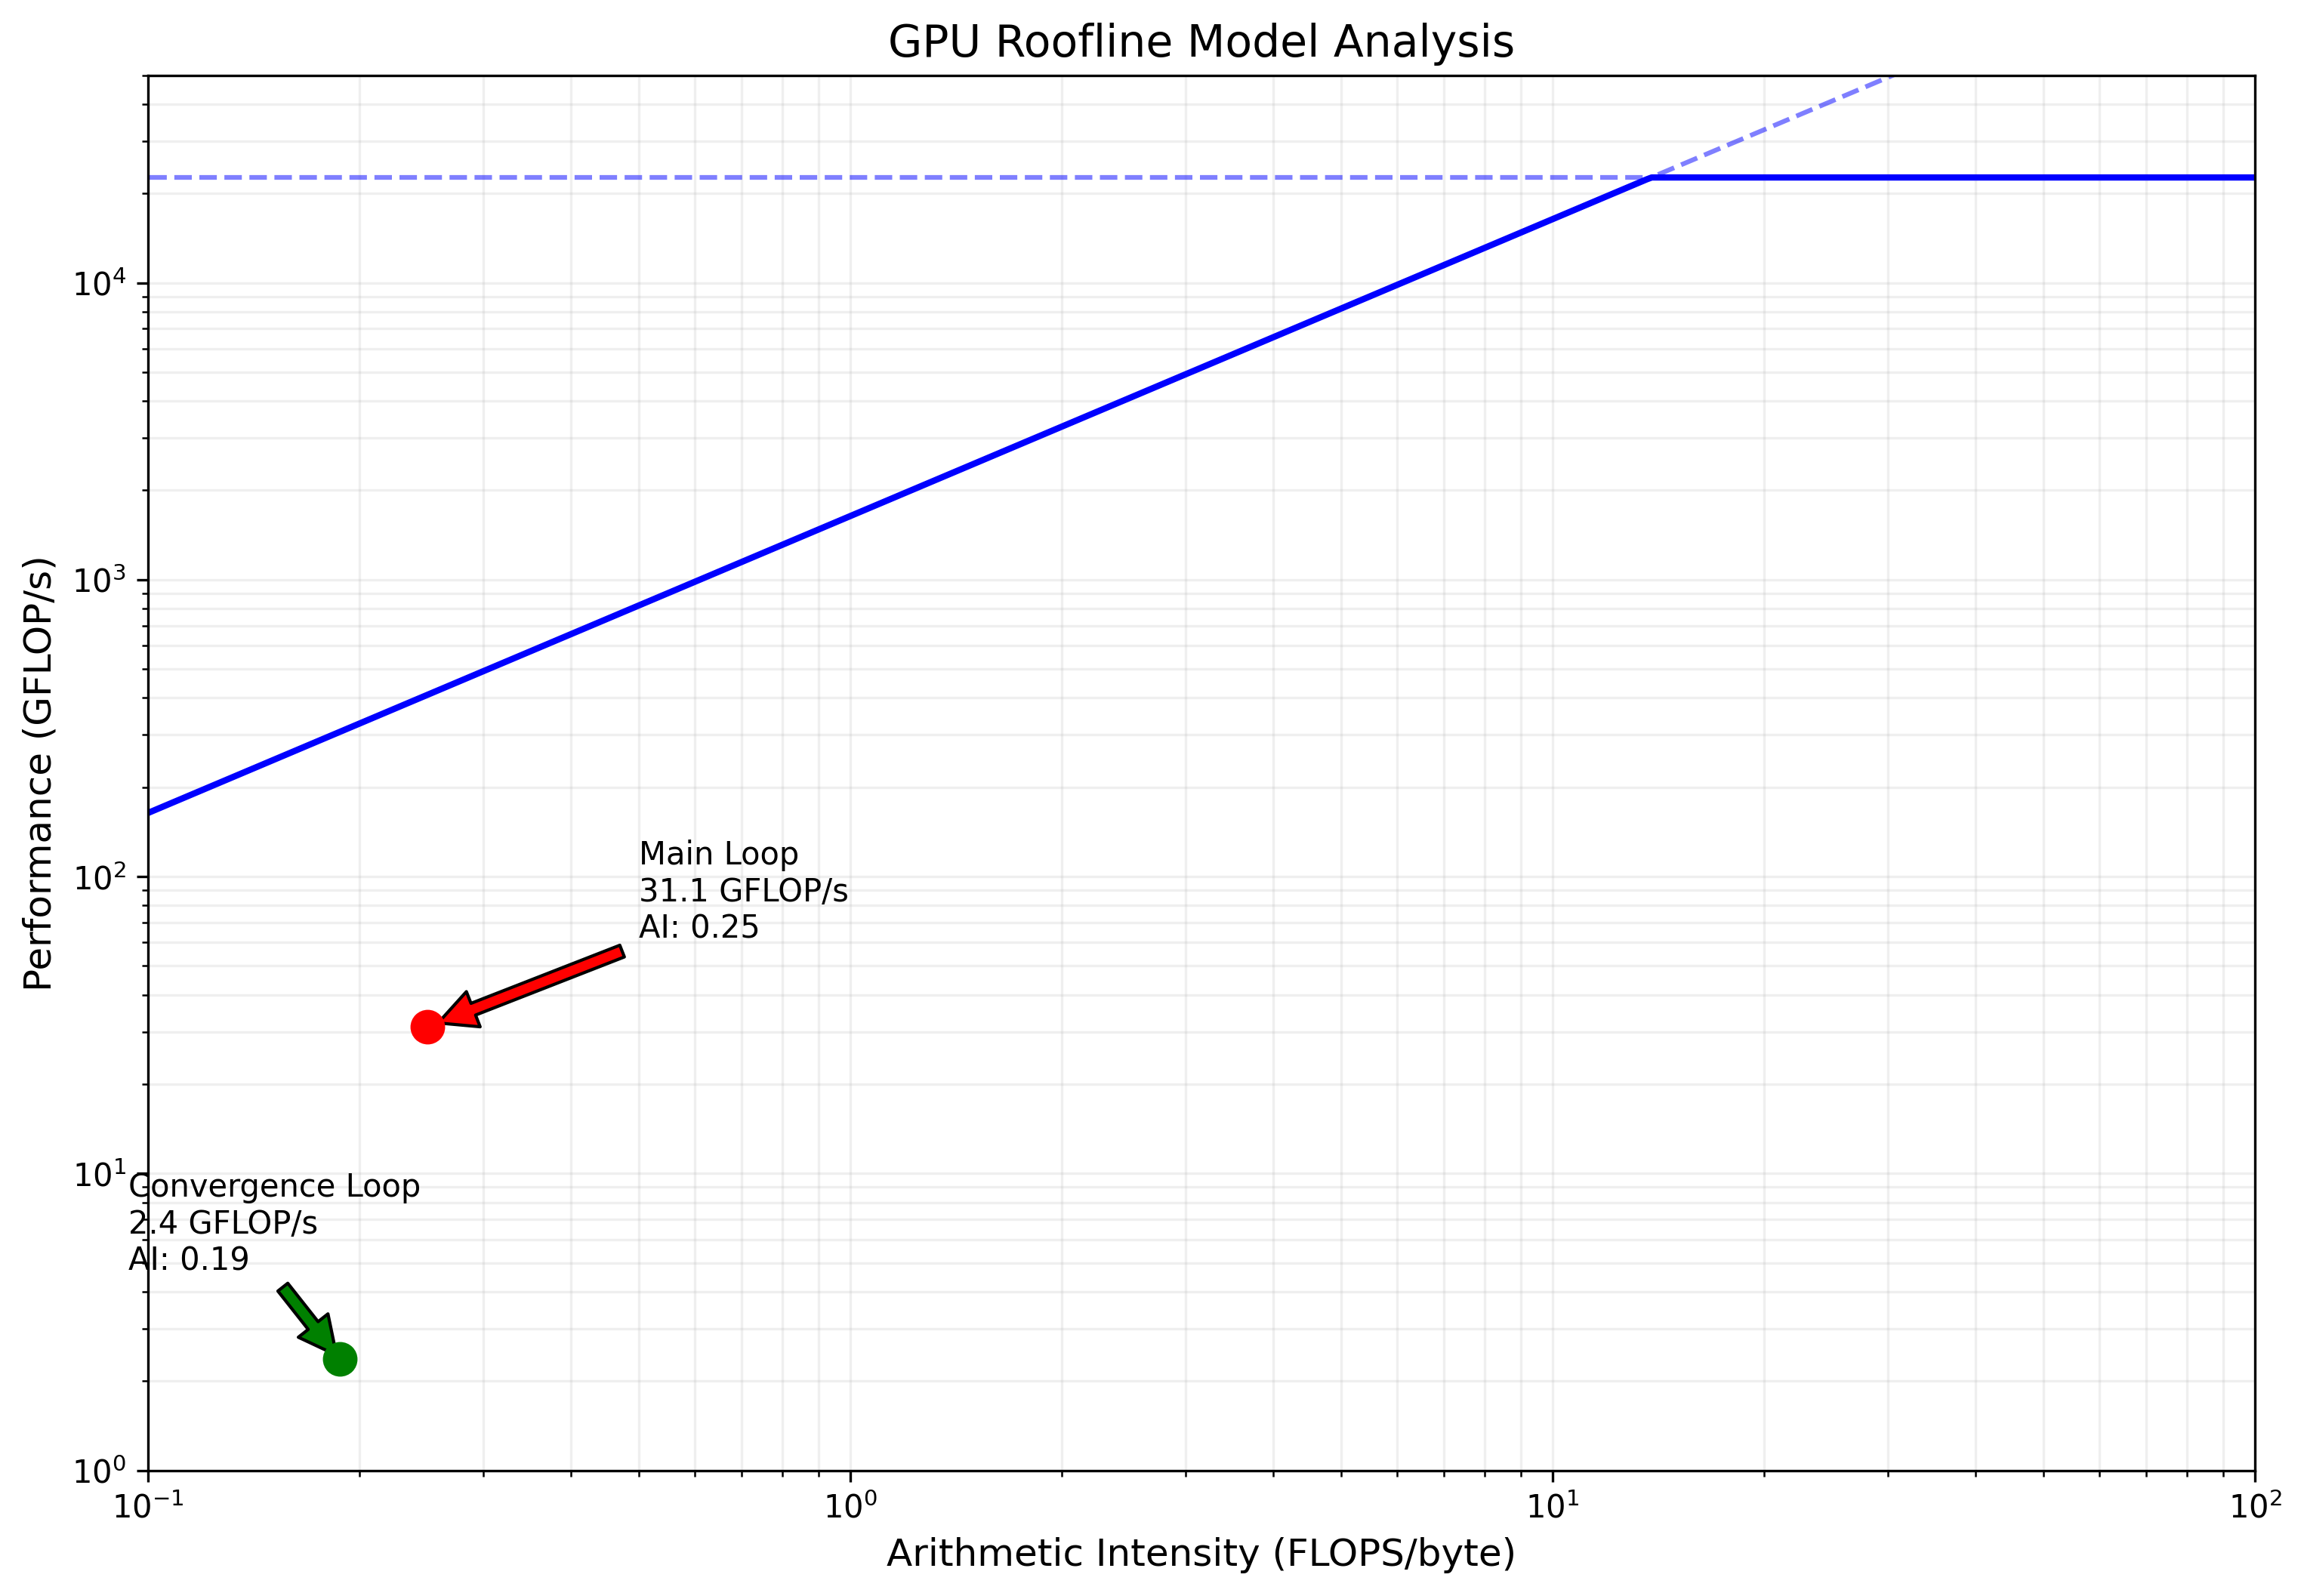
\includegraphics[width=0.8\textwidth]{gpu_roofline_model.png}
    \caption{Roofline model analysis showing performance bounds and achieved performance}
    \label{fig:roofline}
\end{figure}

For the main computation kernel, we observe an arithmetic intensity of 0.25 FLOPS/byte, where each grid point requires 7 floating-point operations and accesses 28 bytes of memory. The kernel achieves a memory bandwidth of 124.723 GB/s, resulting in an effective performance of 31.18 GFLOPS/s.

The convergence check kernel, with its lower arithmetic intensity of 0.1875 FLOPS/byte, achieves a memory bandwidth of 12.6958 GB/s and a performance of 2.38 GFLOPS/s. This lower performance aligns with expectations given the kernel's simpler computational pattern and reduced data reuse opportunities.

\section{Implementation Comparison}

The transition from single to multi-GPU implementation yielded significant performance improvements, with total execution time reducing from 1.47 to 0.49 seconds, representing a 66.7\% improvement. This reduction primarily stems from the distribution of computational load across four GPUs. The iteration count comparison between implementations (13,471 vs 4,453) suggests consistent numerical behavior across both approaches.

A detailed breakdown of the multi-GPU execution time reveals important performance characteristics. While pure computation time is only 0.0627 seconds, additional overhead comes from memory transfers (0.1496 seconds), MPI communication (0.0148 seconds), and convergence checks (0.2073 seconds). This breakdown highlights that in distributed GPU computing, the actual computation represents only a small fraction of the total execution time.

The aggregate memory bandwidth achieved in the multi-GPU implementation (136.464 GB/s) exceeded that of the single-GPU implementation (124.723 GB/s), demonstrating effective utilization of the distributed memory architecture. However, the significant time spent on convergence checks (0.2073 seconds) indicates a potential area for future optimization.

\section{Conclusions}

Our investigation demonstrates the complex interplay between hardware capabilities, algorithmic choices, and implementation strategies in GPU-accelerated scientific computing. Both implementations successfully solved the 2D Poisson equation, with the multi-GPU version showing superior performance despite the modest problem size.

The memory-bound nature of our implementations, revealed through roofline analysis, suggests that future performance improvements would likely come from algorithmic changes rather than hardware optimization alone. Future work could explore implementing more sophisticated preconditioners, investigating 2D domain decomposition strategies, or integrating GPU-aware MPI to reduce communication overhead.

\end{document}